% !TEX root = ../../../main.tex

\toggletrue{image}
\togglefalse{imagehover}
\chapterimage{493-drawing-stars-0}
\chapterimagetitle{\uppercase{Petersen-Graph}}
\chapterimageurl{spikedmath.com}

\chapter{Graphen}
\label{chapter-graphen}

Mit Graphen können wir eine Strassenkarte darstellen. Auch Verbindungen zwischen Profilen in sozialen Netzwerken (\say{Wer ist mit wem befreundet?} oder \say{Welche Personen folgen meinem Account?}) lassen sich mithilfe von Graphen modellieren. In diesem Kapitel beschäftigen wir uns mit den Grundlagen der Graphen. Die Lernziele für dieses Kapitel lauten:

\newcommand{\graphenLernziele}{
\protect\begin{todolist}
\item Sie erklären die Grundbegriffe eines Graphen an einem Beispiel.
\item Sie notieren einen gerichteten/ungerichteten/gewichteten Graphen formal.
\item Sie zeichnen einen gerichteten/ungerichteten/gewichteten Graphen grafisch.
\end{todolist}
}

\lernziel{\autoref{chapter-graphen}, \nameref{chapter-graphen}}{\protect\graphenLernziele}

\graphenLernziele

\begin{hinweis}
Wir erklären die Begriffe in den folgenden Abschnitten an beliebigen Graphen ohne einen Bezug zu realen Situationen. Dies bedeutet, die Graphen repräsentieren zum Beispiel weder eine konkrete Strassenkarte noch ein soziales Netzwerk. Es geht hauptsächlich darum, sich die Konzepte der Graphentheorie anzueignen. An einer anderen Stelle werden die Graphen dann für konkrete Algorithmen eingesetzt.
\end{hinweis}

\section{Grundlagen}

Ein Graph besteht aus \textbf{Knoten} (eng. vertices; Einzahl: vertex) und \textbf{Kanten} (eng. edges). Knoten werden typischerweise als Punkte gezeichnet. Die Verbindung zwischen zwei Knoten wird als Kante bezeichnet. \autoref{figure-graph-1} zeigt ein Beispiel.

\begin{figure}[ht]
\centering
\begin{minipage}{0.3\textwidth}
	\begin{tikzpicture}
    \node[circle, fill, inner sep=2pt, label={west:$v_1$}] (v1) at (0,0) {};
    \node[circle, fill, inner sep=2pt, label={north:$v_2$}] (v2) at (2,0) {};
    \node[circle, fill, inner sep=2pt, label={north:$v_3$}] (v3) at (1,-1) {};
    \node[circle, fill, inner sep=2pt, label={east:$v_4$}] (v4) at (2,-1) {};
    \node (e1) at (1, 1) {(gerichtete) Kante};
    \node (e2) at (1, 0) {};
    \path[->, >=stealth', thick] (v1) edge (v2);
    \path[->, >=stealth', thick] (v2) edge (v3);
    \path[->, >=stealth', thick] (v2) edge (v4);
    \path[->, >=stealth', thick] (v4) edge[bend left=90] (v1);
    \path[->, >=stealth', shorten >=0.1cm] (e1) edge (e2);
\end{tikzpicture}
\caption{Gerichteter Graph mit 4 Knoten und 4 Kanten.}
\label{figure-graph-1}
\end{minipage}
\hfill
\begin{minipage}{0.65\textwidth}
	\centering	
	\begin{tikzpicture}
    \node[circle, fill, inner sep=2pt, label={west:$v_1$}] (v1) at (0,0) {};
    \node[circle, fill, inner sep=2pt, label={north:$v_2$}] (v2) at (2,0) {};
    \node[circle, fill, inner sep=2pt, label={north:$v_3$}] (v3) at (4,0) {};
    \node[circle, fill, inner sep=2pt, label={east:$v_4$}] (v4) at (6,0) {};
    \node[circle, fill, inner sep=2pt, label={west:$v_5$}] (v5) at (1,-1) {};
    \node[circle, fill, inner sep=2pt, label={east:$v_6$}] (v6) at (0,-2) {};
    \node[circle, fill, inner sep=2pt, label={east:$v_7$}] (v7) at (5,-1) {};
    \node[circle, fill, inner sep=2pt, label={east:$v_8$}] (v8) at (5,-2) {};
    \node[text width=2cm] (Knoten) at (8, -1) {Knoten \newline (eng. vertex)};
    \node (e1) at (3, -3) {Kante (eng. edge)};
    \node (e2) at (3, -1) {};
    \path[->, >=stealth', shorten >=0.25cm] (Knoten) edge[bend left] (v4);
    \path[->, >=stealth', shorten >=0.1cm] (e1) edge (e2);
    \path[thick] (v1) edge (v2);
    \path[thick] (v1) edge (v5);
    \path[thick] (v2) edge (v3);
    \path[thick] (v2) edge (v5);
    \path[thick] (v3) edge (v4);
    \path[thick] (v3) edge (v7);
    \path[thick] (v5) edge (v7);
    \path[thick] (v7) edge (v8);
    \path[thick] (v5) edge (v6);
	\end{tikzpicture}
	\caption{Ungerichteter Graph mit 8 Knoten und 9 Kanten.}
\label{figure-graph-2}
\end{minipage}
\end{figure}

Entweder besitzen alle Kanten an einem Ende eine Pfeilspitze (wie in \autoref{figure-graph-1}), dann sprechen wir von einem \textbf{gerichteten Graphen} oder keine Kante besitzt eine Pfeilspitze (wie in \autoref{figure-graph-2}) dann handelt es sich um einen \textbf{ungerichteten Graphen}.

\section{Gerichtete Graphen}

Ein gerichteter Graph (eng. directed graph) ist ein Graph, bei dem jede Kante eine \textbf{Richtung} besitzt. Ein Beispiel ist in \autoref{figure-graph-3} zu sehen. Die Richtung wird durch eine Pfeilspitze dargestellt. Die Idee ist, dass wir nur in die Pfeilrichtung \say{fahren} dürfen (z.B. die Kante soll eine Einbahnstrasse darstellen) oder sich Güter ausschliesslich in diese Richtung \say{bewegen} können. Kanten mit einer Pfeilspitze werden \textbf{gerichtete Kanten} genannt.

\begin{figure}[ht]
\centering
\begin{minipage}{0.45\textwidth}
\centering
\begin{tikzpicture}
    \node[circle, fill, inner sep=2pt, label={west:$v_1$}] (v1) at (0,0) {};
    \node[circle, fill, inner sep=2pt, label={west:$v_2$}] (v2) at (0,1) {};
    \node[circle, fill, inner sep=2pt, label={west:$v_3$}] (v3) at (0,2) {};
    \node[circle, fill, inner sep=2pt, label={east:$v_4$}] (v4) at (1,0) {};
    \node[circle, fill, inner sep=2pt, label={east:$v_5$}] (v5) at (1,2) {};
    \path[->, >=stealth', thick] (v1) edge (v2);
    \path[->, >=stealth', thick] (v1) edge (v4);
    \path[->, >=stealth', thick] (v2) edge (v3);
    \path[->, >=stealth', thick] (v2) edge (v5);
    \path[->, >=stealth', thick] (v3) edge (v5);
    \path[->, >=stealth', thick] (v4) edge (v5);
    \path[->, >=stealth', thick] (v4) edge (v2);
\end{tikzpicture}
\caption{Beispielgraph 1}
\label{figure-graph-3}
\end{minipage}
\hfill
\begin{minipage}{0.45\textwidth}
\centering
\begin{tikzpicture}
    \node[circle, fill, inner sep=2pt, label={west:$v_1$}] (v1) at (-0.5,1) {};
    \node[circle, fill, inner sep=2pt, label={west:$v_2$}] (v2) at (0,0) {};
    \node[circle, fill, inner sep=2pt, label={east:$v_3$}] (v3) at (2,1) {};
    \node[circle, fill, inner sep=2pt, label={south:$v_4$}] (v4) at (1,0.5) {};
    \node[circle, fill, inner sep=2pt, label={east:$v_5$}] (v5) at (0.5,2) {};
    \path[->, >=stealth', thick] (v1) edge (v2);
    \path[->, >=stealth', thick] (v1) edge (v4);
    \path[->, >=stealth', thick] (v2) edge (v3);
    \path[->, >=stealth', thick] (v2) edge (v5);
    \path[->, >=stealth', thick] (v3) edge (v5);
    \path[->, >=stealth', thick] (v4) edge (v5);
    \path[->, >=stealth', thick] (v4) edge (v2);
\end{tikzpicture}
\caption{Beispielgraph 2}
\label{figure-graph-4}
\end{minipage}
\end{figure} 

\autoref{figure-graph-4} zeigt ebenfalls einen gerichteten Graphen. Es ist der gleiche Graph wie in \autoref{figure-graph-3}. Die Knoten wurden einfach an einer anderen Stelle gezeichnet. Dies spielt bei der grafischen Darstellung eines Graphen keine Rolle. Wichtig sind nur die Anzahl der Knoten und die Kanten zwischen den Knoten. Die beiden Graphen sind also identisch.

\subsection{Formale Notation}

Einen gerichteten Graphen können wir formal notieren. Der gerichtete Graph aus \autoref{figure-graph-3} wird wie folgt beschrieben:
\begin{align*}
G & = (V, E) & V & = \{v_1, v_2, v_3, v_4, v_5\} \\
& & E & = \{(v_1, v_2), (v_1, v_4), (v_2, v_3), (v_2, v_5), (v_3, v_5), (v_4, v_5), (v_4, v_2)\}
\end{align*}
Der Graph $G$ ist ein Paar aus einer \textbf{Knotenmenge} $V$ (vertices) und einer \textbf{Kantenmenge} $E$ (edges). Die Knotenmenge $V$ besteht aus einer Menge von Knoten $v_i$ und die Kantenmenge $E$ besteht aus einer Menge von \textbf{Knotenpaaren} $(v_i, v_j)$. Die Reihenfolge der Knoten in einem Knotenpaar ist wichtig:

\begin{figure}[htb]
\centering
\begin{minipage}[c]{0.45\textwidth}
\centering
\begin{tikzpicture}
    \node[circle,fill,inner sep=2pt,label={north west:$v_1$}] (v1) at (0,2) {};
    \node[circle,fill,inner sep=2pt,label={north east:$v_2$}] (v2) at (1,2) {};
    \path[->, >=stealth', thick] (v1) edge (v2);
\end{tikzpicture}
\caption*{$(v_1, v_2)$}
\end{minipage}
\begin{minipage}[c]{0.45\textwidth}
\centering
\begin{tikzpicture}
    \node[circle,fill,inner sep=2pt,label={north west:$v_1$}] (v1) at (0,2) {};
    \node[circle,fill,inner sep=2pt,label={north east:$v_2$}] (v2) at (1,2) {};
    \path[->, >=stealth', thick] (v2) edge (v1);
\end{tikzpicture}
\caption*{$(v_2, v_1)$}
\end{minipage}
\caption*{$(v_1, v_2) \neq (v_2, v_1)$}
\end{figure}

\section{Ungerichtete Graphen}

In einem ungerichteten Graphen (eng. undirected graph) besitzt \textbf{keine} Kante eine Pfeilspitze. \autoref{figure-graph-6} zeigt ein Beispiel. Die Idee von ungerichteten Kanten ist es, dass es keine Einschränkungen in der \say{Bewegungsrichtung} gibt.

\begin{figure}[htb]
\centering
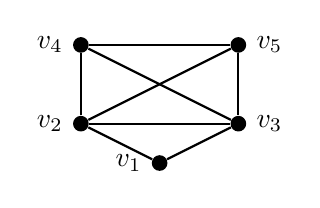
\begin{tikzpicture}
    \node[circle, fill, inner sep=2pt, label={west:$v_1$}] (v1) at (0,0.5) {};
    \node[circle, fill, inner sep=2pt, label={west:$v_2$}] (v2) at (-1,1) {};
    \node[circle, fill, inner sep=2pt, label={east:$v_3$}] (v3) at (1,1) {};
    \node[circle, fill, inner sep=2pt, label={west:$v_4$}] (v4) at (-1,2) {};
    \node[circle, fill, inner sep=2pt, label={east:$v_5$}] (v5) at (1,2) {};
    \path[thick] (v1) edge (v2);
    \path[thick] (v1) edge (v3);
    \path[thick] (v2) edge (v3);
    \path[thick] (v2) edge (v4);
    \path[thick] (v2) edge (v5);
    \path[thick] (v3) edge (v4);
    \path[thick] (v3) edge (v5);
    \path[thick] (v4) edge (v5);
\end{tikzpicture}
\caption{Ein ungerichteter Graph mit 5 Knoten und 8 Kanten.}
\label{figure-graph-6}
\end{figure}

Die grafische Darstellung unterscheidet sich sonst nicht von gerichteten Graphen. Die Position der Knoten bei der grafischen Darstellung spielt auch hier keine Rolle.

\subsection{Formale Notation}

Einen ungerichteten Graphen können wir formal notieren. Der ungerichtete Graph aus \autoref{figure-graph-6} wird wie folgt beschrieben:
\begin{align*}
G & = (V, E) & V & = \{v_1, v_2, v_3, v_4\} \\
& & E & = \{\{v_1, v_2\},\{v_1, v_3\},\{v_2, v_3\},\{v_2, v_4\},\{v_2, v_5\},\{v_3, v_4\},\{v_3, v_5\},\{v_4, v_5\}\}
\end{align*}
Die Kantenmenge $E$ besteht aus einer Menge von \textbf{Knotenmengen} $\{v_i, v_j\}$. Die Reihenfolge der Knoten in einer Knotenmenge ist \textbf{nicht} wichtig:

\begin{figure}[htb]
\centering
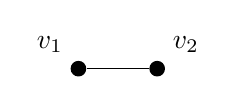
\begin{tikzpicture}
    \node[circle, fill, inner sep=2pt, label={north west:$v_1$}] (v1) at (0,0) {};
    \node[circle, fill, inner sep=2pt, label={north east:$v_2$}] (v2) at (1,0) {};
    \path (v1) edge (v2);
\end{tikzpicture}
\caption*{$\{v_1, v_2\} = \{v_2, v_1\}$}
\end{figure}

\begin{important}
Vergleichen wir die formale Notation von \textbf{gerichteten} und \textbf{ungerichteten Graphen}, dann unterscheiden sich die beiden Notationen nur in der \textbf{Kantenmenge}.
\end{important}

\section{Gewichtete Graphen}

Ordnen wir jeder \textbf{Kante} in einem Graphen eine Zahl zu, dann sprechen wir von einem gewichteten Graphen (eng. weighted graph). Die Zahlen an den Kanten nennen wir \textbf{Gewichte}. \autoref{figure-graph-8} zeigt einen ungerichteten Graphen mit Gewichten.

\begin{figure}[htb]
\centering
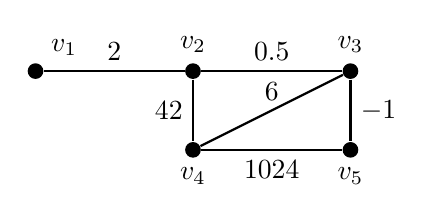
\begin{tikzpicture}
    \node[circle, fill, inner sep=2pt, label={north east:$v_1$}] (v1) at (0,0) {};
    \node[circle, fill, inner sep=2pt, label={north:$v_2$}] (v2) at (2,0) {};
    \node[circle, fill, inner sep=2pt, label={north:$v_3$}] (v3) at (4,0) {};
    \node[circle, fill, inner sep=2pt, label={south:$v_4$}] (v4) at (2,-1) {};
    \node[circle, fill, inner sep=2pt, label={south:$v_5$}] (v5) at (4,-1) {};
    \path[thick] (v1) edge node[above] {$2$} (v2);
    \path[thick] (v2) edge node[above] {$0.5$} (v3);
    \path[thick] (v2) edge node[left] {$42$} (v4);
    \path[thick] (v3) edge node[above] {$6$} (v4);
    \path[thick] (v3) edge node[right] {$-1$} (v5);
    \path[thick] (v4) edge node[below] {$1024$} (v5);
\end{tikzpicture}
\caption{Der gerichtete und gewichtete Graph besitzt 5 Knoten, 6 Kanten und 6 Gewichte.}
\label{figure-graph-8}
\end{figure}

Die Gewichte in einem Graphen können etwa Entfernungen in Kilometer sein, Fahrtkosten in einer Währung oder Fahrtzeiten in Minuten.

\subsection{Formale Notation}

Einen gewichteten Graphen können wir formal notieren. Der ungerichtete und gewichtete Graph aus \autoref{figure-graph-8} wird wie folgt beschrieben:
\begin{align*}
G &= (V, E, w) & V &= \{v_1, v_2, v_3, v_4, v_5\} & E &= \{\{v_1, v_2\}, \{v_2, v_4\}, \{v_2, v_3\}, \{v_3, v_4\}, \{v_3, v_5\}, \{v_4, v_5\}\}
\end{align*}
Die Gewichte für die Kanten werden wie folgt notiert:
\begin{align*}
w(\{v_1, v_2\}) &= 2 & w(\{v_2, v_4\}) &= 42 & w(\{v_3, v_5\}) &= -1 \\
w(\{v_2, v_3\}) &= 0.5 & w(\{v_3, v_4\}) &= 6 & w(\{v_4, v_5\}) &= 1024
\end{align*}
Wir bezeichnen mit $w$ die \textbf{Gewichtsfunktion}, welche jeder Kante ein Gewicht zuordnet.

\subsection{Distanzgraphen}

Modellieren wir eine Strassenkarte als Graphen, dann kommen Distanzgraphen zum Einsatz, da alle Verbindungen typischerweise nur positive Werte besitzen.

\begin{definition}[Distanzgraph]
	Falls ein gewichteter Graph nur \textbf{positive Gewichte} besitzt, dann handelt es sich um einen Distanzgraphen.
\end{definition}

\section{Aufgaben}

\begin{enumerate}

\item Notieren Sie den Graphen aus \autoref{figure-graph-5} formal.

\begin{figure}[H]
\centering
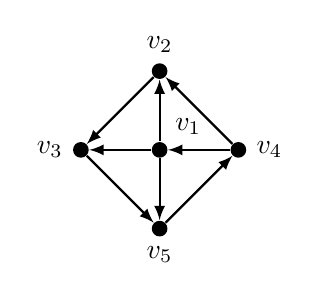
\begin{tikzpicture}
    \node[circle, fill, inner sep=2pt, label={north east:$v_1$}] (v1) at (0,0) {};
    \node[circle, fill, inner sep=2pt, label={north:$v_2$}] (v2) at (0,1) {};
    \node[circle, fill, inner sep=2pt, label={west:$v_3$}] (v3) at (-1,0) {};
    \node[circle, fill, inner sep=2pt, label={east:$v_4$}] (v4) at (1,0) {};
    \node[circle, fill, inner sep=2pt, label={south:$v_5$}] (v5) at (0,-1) {};
    \path[-latex, thick] (v1) edge (v2);
    \path[-latex, thick] (v1) edge (v3);
    \path[latex-, thick] (v1) edge (v4);
    \path[-latex, thick] (v1) edge (v5);
    \path[-latex, thick] (v2) edge (v3);
    \path[-latex, thick] (v3) edge (v5);
    \path[-latex, thick] (v4) edge (v2);
    \path[-latex, thick] (v5) edge (v4);
\end{tikzpicture}
\caption{Graph mit $5$ Knoten.}
\label{figure-graph-5}
\end{figure}

\fillwithgrid{1in}

\item Stellen Sie den Graphen $G = (V, E)$ grafisch dar. Es gilt:
\begin{align*}
V & = \{v_1,v_2,v_3,v_4\} \\
E & = \{(v_1,v_2),(v_2,v_3),(v_3,v_4),(v_4,v_1),(v_2,v_4),(v_1,v_3)\}
\end{align*}

\fillwithgrid{2in}

\item Notieren Sie den Graphen aus \autoref{figure-graph-7} formal.

\begin{figure}[ht]
\centering
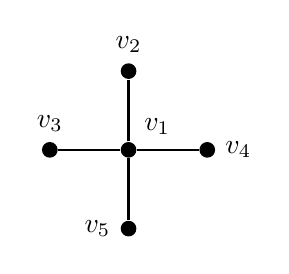
\begin{tikzpicture}
    \node[circle, fill, inner sep=2pt, label={north east:$v_1$}] (v1) at (0,0) {};
    \node[circle, fill, inner sep=2pt, label={north:$v_2$}] (v2) at (0,1) {};
    \node[circle, fill, inner sep=2pt, label={north:$v_3$}] (v3) at (-1,0) {};
    \node[circle, fill, inner sep=2pt, label={east:$v_4$}] (v4) at (1,0) {};
    \node[circle, fill, inner sep=2pt, label={west:$v_5$}] (v5) at (0,-1) {};
    \path[thick] (v1) edge (v2);
    \path[thick] (v1) edge (v3);
    \path[thick] (v1) edge (v4);
    \path[thick] (v1) edge (v5);
\end{tikzpicture}
\caption{Ein Graph mit $5$ Knoten.}
\label{figure-graph-7}
\end{figure}

\fillwithgrid{\stretch{1}}

\newpage

\item Stellen Sie den Graphen $G = (V, E)$ grafisch dar. Es gilt:
\begin{align*}
V & = \{v_1,v_2,v_3,v_4,v_5\} \\
E & =\{\{v_1,v_2\},\{v_2,v_3\},\{v_2,v_4\},\{v_4,v_5\},\{v_3,v_5\}\}
\end{align*}

\fillwithgrid{2in}

\item Notieren Sie formal für den Graphen aus \autoref{figure-graph-9} die Knotenmenge $V$, die Kantenmenge $E$ sowie die Gewichte für jede Kante $e \in E$.

\begin{figure}[htb]
\centering
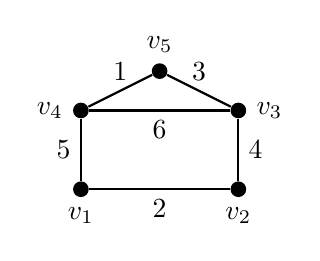
\begin{tikzpicture}
    \node[circle, fill, inner sep=2pt, label={south:$v_1$}] (v1) at (0,0) {};
    \node[circle, fill, inner sep=2pt, label={south:$v_2$}] (v2) at (2,0) {};
    \node[circle, fill, inner sep=2pt, label={east:$v_3$}] (v3) at (2,1) {};
    \node[circle, fill, inner sep=2pt, label={west:$v_4$}] (v4) at (0,1) {};
    \node[circle, fill, inner sep=2pt, label={north:$v_5$}] (v5) at (1,1.5) {};
    \path[thick] (v1) edge node[below] {$2$} (v2);
    \path[thick] (v2) edge node[right] {$4$} (v3);
    \path[thick] (v3) edge node[below] {$6$} (v4);
    \path[thick] (v4) edge node[left] {$5$} (v1);
    \path[thick] (v4) edge node[above] {$1$} (v5);
    \path[thick] (v3) edge node[above] {$3$} (v5);
\end{tikzpicture}
\caption{Ein bewerteter Graph mit $5$ Knoten.}
\label{figure-graph-9}
\end{figure}

\fillwithgrid{1in}

\item Stellen Sie den Graphen $G = (V, E, w)$ mit $V=\{v_1,v_2,v_3\}$, $E=\{\{v_1,v_2\},\{v_2,v_3\},\{v_3,v_1\}\}$ und den Gewichten $w(\{v_1,v_2\})=8, w(\{v_2,v_3\})=-1, w(\{v_3,v_1\})=3$ grafisch dar. Handelt es sich um einen Distanzgraphen? Begründen Sie Ihre Antwort.

\fillwithgrid{2in}

\end{enumerate}
